\section{Quadrics of revolution}
\label{sec:conic}

\newcommand\Sin{\ensuremath{\mathcal{S}}}
\newcommand\Cos{\ensuremath{\mathcal{C}}}
\newcommand\Cot{\ensuremath{\mathcal{T}}}

For an arbitrary surface of revolution, application of
equations~(\ref{eq:tanphi}, \ref{eq:tangential}) to determine the
projected shape of the tangent line is not straightforward and in
general requires numerical techniques.  However, analytical results
can be found for the important class of surfaces known as
\textit{quadrics of revolution} \citep{Goldman:1983a, Gfrerrer:2009a},
which are formed by rotating a conic section plane curve about its
symmetry axis.  Examples are the sphere, spheroids (oblate and
prolate), and right circular paraboloids and hyperboloids.\footnote{We
  consider only the case of a single sheet of a 2-sheet hyperboloid or
  paraboloid.}  We ignore the degenerate cases of cylinders, cones,
and pairs of parallel planes.  While mathematically simple, these
quadrics are sufficiently flexible that they can provide a useful
approximation to more complex bow shock shapes. 

%The 
%In this section we will analyze the case where the resultant shape  of the bow shock is a conic curve (circle, ellipse, parabola or hyperbola).
%These curves are mathematical simple to model and give us a good reference to understand the effects of the projection effects
%described in the last section on other bow shocks. The source of the inner wind is located at the origin, and the center of the conic is located at
%a distance $x_0$ from the source.

%Instead of the excentricity, we utilize the parameter $\theta_c$ to characterize the different curves, where
%$\tan\theta_c = \frac{b}{a}$,  $b$ and $a$ are the typical parameters of conics. A positive value for $\theta_c$ indicates that the given curve is a closed one, i.e
%an ellipse, while a negative value indicates that is an hyperbola. %Insert figures if neccesary  
\begin{figure*}
\setlength\tabcolsep{0pt}
\begin{tabular}{cc}
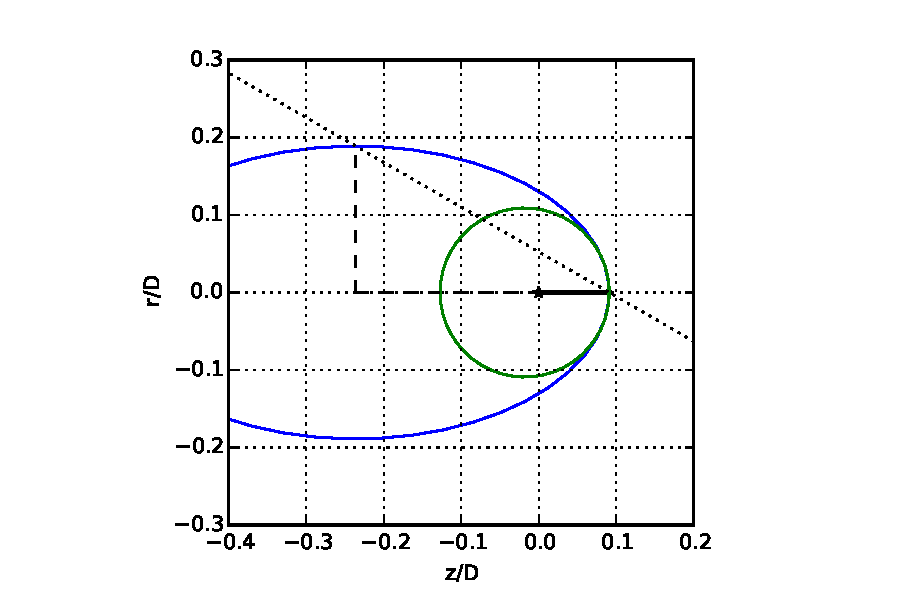
\includegraphics[height=0.54\linewidth, trim=30 0 30 0, clip]{ellipse_py} &
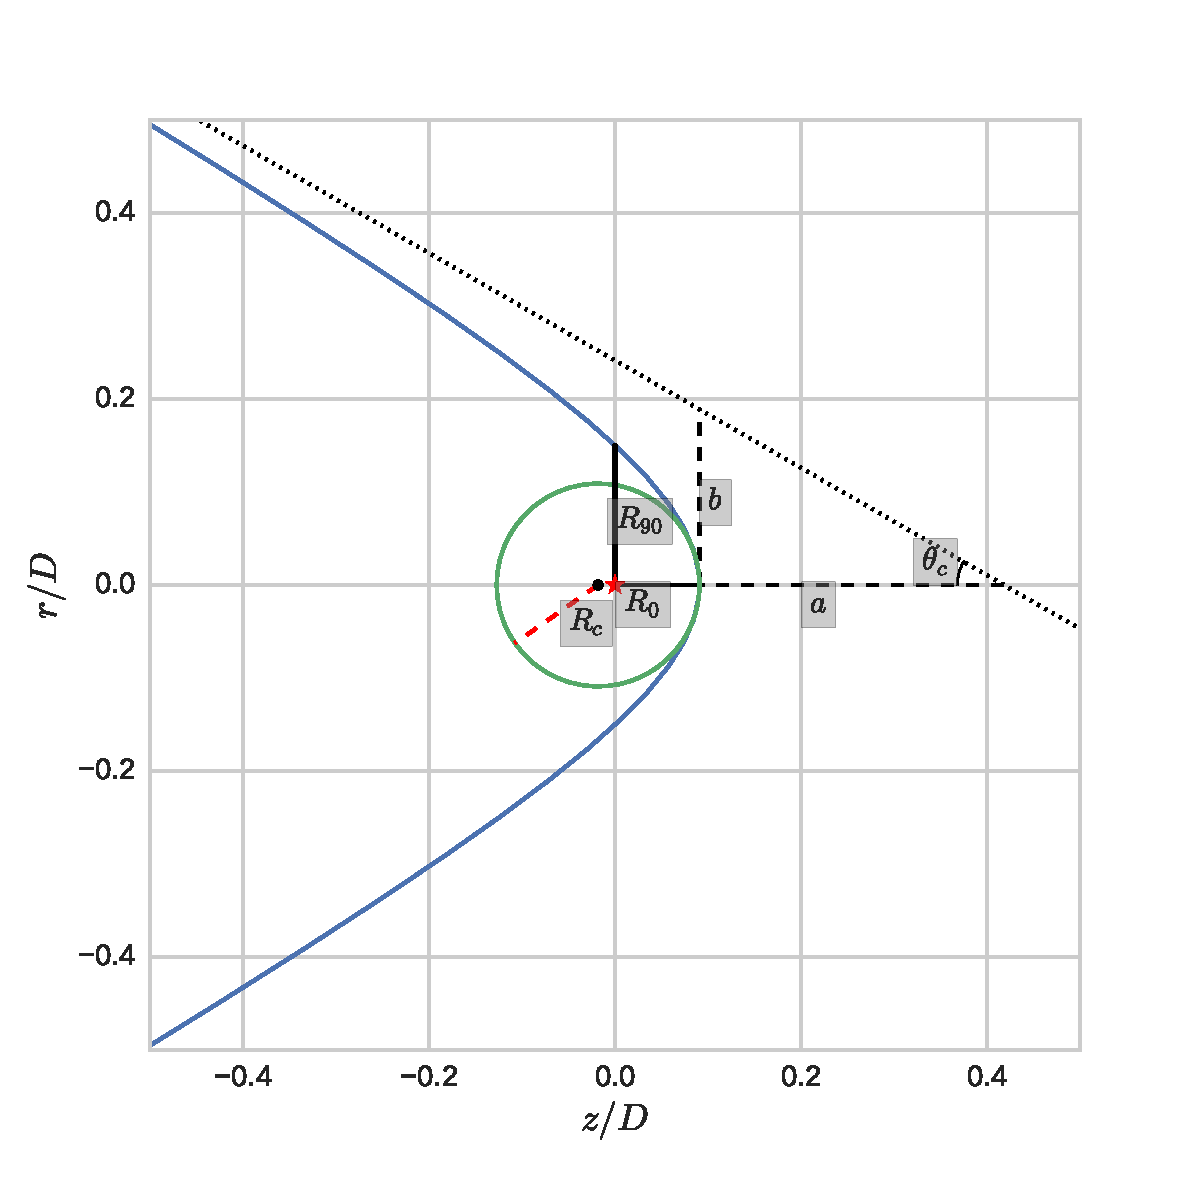
\includegraphics[height=0.54\linewidth, trim=60 0 70 0, clip]{hyperbola_py}
\end{tabular}
\label{fig:conics}
\caption{Schematic representation of conic like bowshocks: A) Ellipse and B) Hyperbola.
  The center of the conic is located at a distance $x_0=R_0-a$ from the origin at the $x$ axis 
  The radius of curvature at the axis is $R_c$, and $R_{90}$ is t he radius of the conic in the
  perpendicular direction to $R_0$.
}
\end{figure*}
\begin{figure}
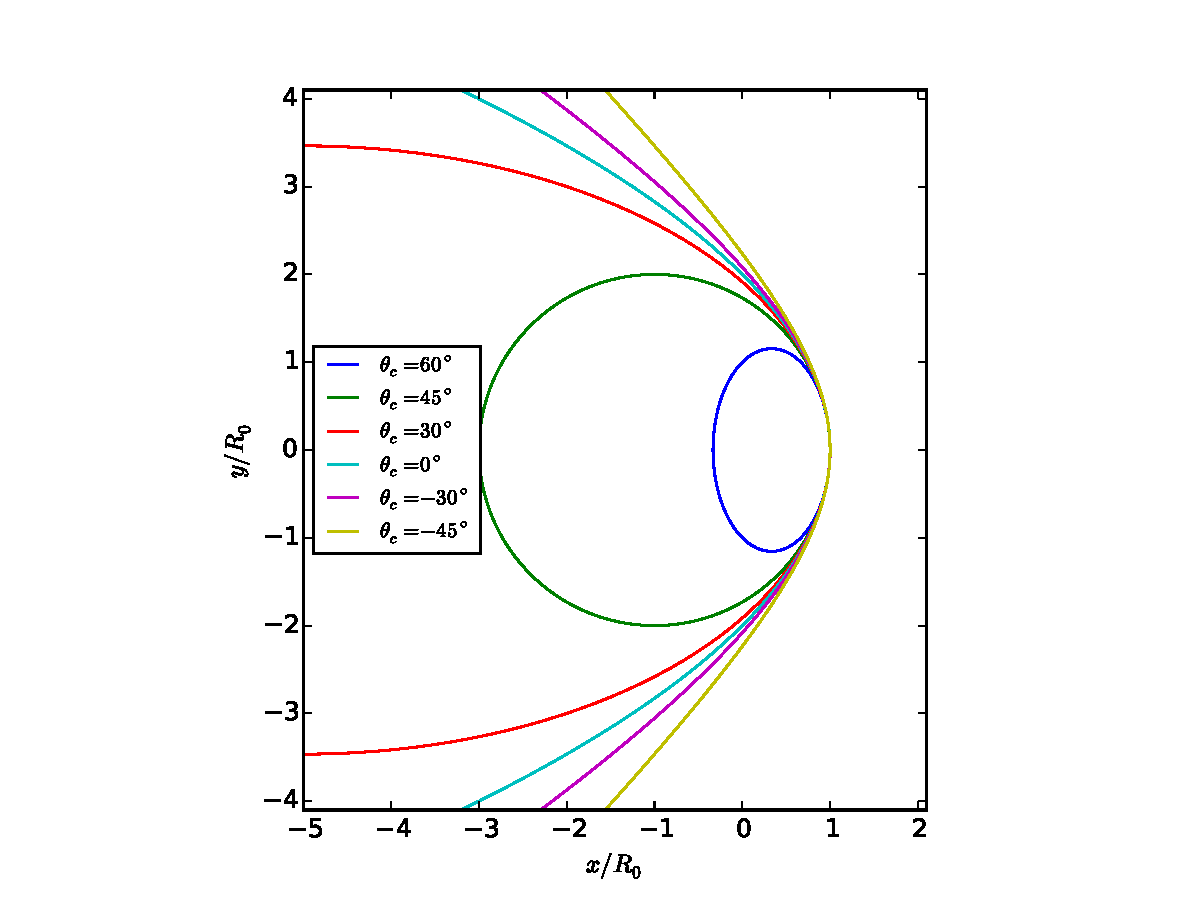
\includegraphics[width=\linewidth]{conic1}
\caption{Example of a family of conic sections, all with the same
  radius of curvature at their apex (marked by white dot) on the
  \(x\)~axis: \(R_c = 2 R_0\). The parameter
  $\theta_c = \pm \tan^{-1} b/a$ describes the family, with negative
  values corresponding to hyperbolae.}
\label{fig:conics-family}
\end{figure}

Due to the similarities between the parametrization of the ellipse and the hyperbola, we can do the following parametrization
\footnote{Equations (\ref{eq:par-x}) to (\ref{eq:b-prime}) does not apply for paraboloids. Instead, the parametrization and the
  projected shape are developed in appendix \ref{app:parabola}}:
\begin{align}
x &= a\Cos(t)-x_0 \label{eq:par-x}\\ 
y &= b\Sin(t) \label{eq:par-y}
\end{align}
where:
\begin{align}
\Cos(t) &= \left\lbrace \begin{array}{c}
\cos t ~\mathrm{if~ellipse} \\
\cosh t ~\mathrm{if~hyperbola}
\end{array}\right.\\
\Sin(t) &= \left\lbrace \begin{array}{c}
\sin t ~\mathrm{if~ellipse} \\
\sinh t ~\mathrm{if~hyperbola}
\end{array}\right. \\
-\pi < t < \pi \\
R_0 &= a - x_0 \\
a<0 ~ \mathrm{for~hyperbola}
\end{align}
We have set a whole family of curves with a singular parameter denoted as $\tan\theta_c \equiv \frac{b}{a}$. Positive values of this parameter describe closed curves
(i.e. ellipses) and the negative ones describe open curves (i.e. hyperbolas). Particular cases are $\theta_c =\frac{\pi}{4}$, which describes a circle and $\theta_c=0$, which describes
a parabola.
To determine uniquely a given conic in terms of measurable quantities, we use the set of characteristic radii $(R_0,R_c,R_{90})$ in such way the conic parameters $(a,b,\theta_c)$
could be derived from the former. The transformation between the conic parameters and the characteristic radii are given by:
\begin{align}
R_c &= \frac{b^2}{a} \label{eq:Rc-conic}\\ 
R_{90} &= b\left[\pm\left(1 - \frac{(R_0-a)^2}{a^2}\right)\right]^{1/2}\label{eq:r90-conic}
\end{align}
In (\ref{eq:r90-conic}), the positive sign correspond to an elliptic quadric, while the negative sign to an hyperbolic quadric. The inverse transformation of (\ref{eq:Rc-conic})
and (\ref{eq:r90-conic}) is given by:
\begin{align}
\frac{a}{R_0} &= \frac{A}{2A-B^2} \label{eq:a-conic}\\
\frac{|b|}{R_0} &= \frac{A}{\left|2A-B^2\right|^{1/2}}\\
\tan\theta_c &= \frac{2A-B^2}{\left|B^2 - 2A\right|^{1/2}} \label{eq:thc-conic} \\
\mathrm{where:~} B &\equiv \frac{R_{90}}{R_0} \\
A &\equiv \frac{R_c}{R_0}
\end{align}

\subsection{Plane-of-sky projection of quadric surfaces} 
\begin{figure*}
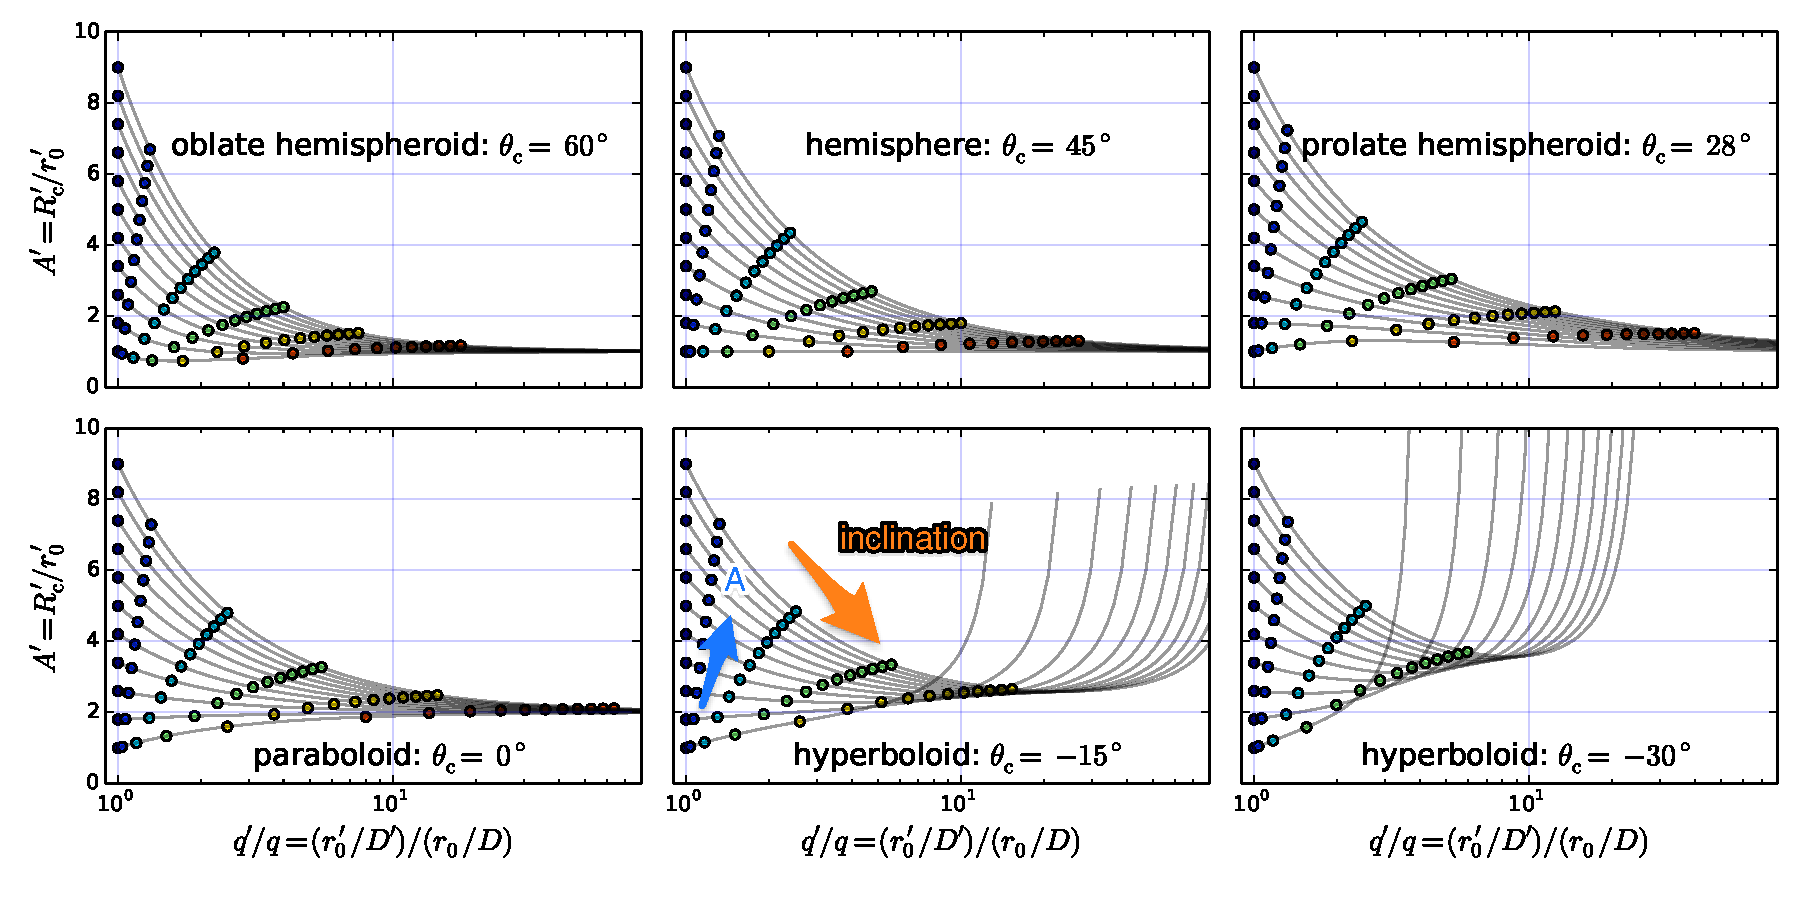
\includegraphics[width=0.9\linewidth]{annotated}
\caption{Projected Radius of curvature vs projected $R_0$ for $\theta_c=60^\circ,45^\circ,28^\circ, 0^\circ,-15^\circ,-30^\circ$. Each colored points represent
the same shape at a different inclination. Being the dark blue the ones with the lower inclination and the red ones with the highest value. For closed shapes, there is
an asymptotic limit for the projected radius of curvature at high inclinations, while for open shapes there is an upper limit for inclination where a tangent line can be observed.}
\label{fig:Apqp}
\end{figure*}

Once the parametrization is done, we can find the apparent shape of
the shell in the observer's frame, following the procedure explained
in section \ref{sec:projection}.  First of all, the intrinsic 3D shape of the shell is given by:
\begin{align}
x &= a\Cos(t)-x_0 \\ 
y &= b\Sin(t)\cos\phi \\
z &=  b\Sin(t)\sin\phi
\end{align}
The azimutal angle where the line of sight is tangent to the shell is given by equation (\ref{eq:tanphi}) and (\ref{eq:alpha}), then:
\begin{align}
\sin\phi_t &= \frac{b}{a}\tan i\Cot(t) 
\end{align}
where:
\begin{align}
\Cot(t) = \left\lbrace \begin{array}{c}
-\cot t ~\mathrm{if~ellipse} \\
\coth t ~\mathrm{if~hyperbola}
\end{array}\right.
\end{align}

We could work in another frame where the origin is located at the conic's center: $(X,Y)$, where $X=x-X_0$ and $Y=y$.
In this frame, we use the transformations (\ref{eq:Trans})  to obtain the apparent shape of the shell:
\begin{align}
X' &= \frac{\Cos(t)}{a\cos i}\left(a^2\cos^2 i \pm b^2\sin^2 i\right)  \label{eq:conic-projected-x}\\
Y' &= b\Sin(t)\left(1-\frac{b^2}{a^2}\tan^2 i\Cot^2(t)\right)^{1/2}
\label{eq:conic-projected-y}
\end{align}


If the apparent shape of the shell in the observer's frame is still the same conic, then, we
can write equations(\ref{eq:conic-projected-x}) and (\ref{eq:conic-projected-y}) as follows:
\begin{align}
X' = a'\Cos( t') \label{eq:conic-projected-x-2} \\
Y' = b'\Sin (t') \label{eq:conic-projected-y-2} . 
\end{align}

Comparing, (\ref{eq:conic-projected-x}), (\ref{eq:conic-projected-x-2}), (\ref{eq:conic-projected-y}) and (\ref{eq:conic-projected-y-2}) we find that
\begin{align}
a' &= \left(a^2\cos^2 i \pm b^2\sin^2 i\right)^{1/2} \\
\Cos(t') &= \frac{a'\Cos(t)}{a\cos i} \\
b' &= b \label{eq:b-prime}
\end{align} 

\begin{align}
D' &= D\cos i \\
R'_0 &= a' - (a-R_0)\cos i \\
R'_0 &= \left(a^2\cos^2 i \pm b^2\sin^2 i\right)^{1/2}  - (a-R_0)\cos i
\end{align}

With  $f(i;\theta_c)\equiv\left(1\pm\tan^2\theta_c\tan^2i\right)^{1/2}$ we find that:
\begin{align}
\frac{R'_0}{D'}=\frac{R_0}{D}\left(1\pm A\cot^2\theta_c(f(i;\theta_c)-1) \right)
\label{eq:qprime}
\end{align}
%Where $A\equiv \frac{R_c}{R_0}$

The Radius of curvature in the observer's frame is given by $R'_c=\frac{b'^2}{a'}$. Then:
\begin{align}
  \frac{R'_c}{R'_0} = \frac{A}{\cos^2 i f(i;\theta_c)\frac{q'}{q}}
  \label{eq:Aprime}
\end{align}
where $q=\frac{R_0}{D}$ and $q' = \frac{R'_0}{D'}$. 
% \begin{figure*}
% 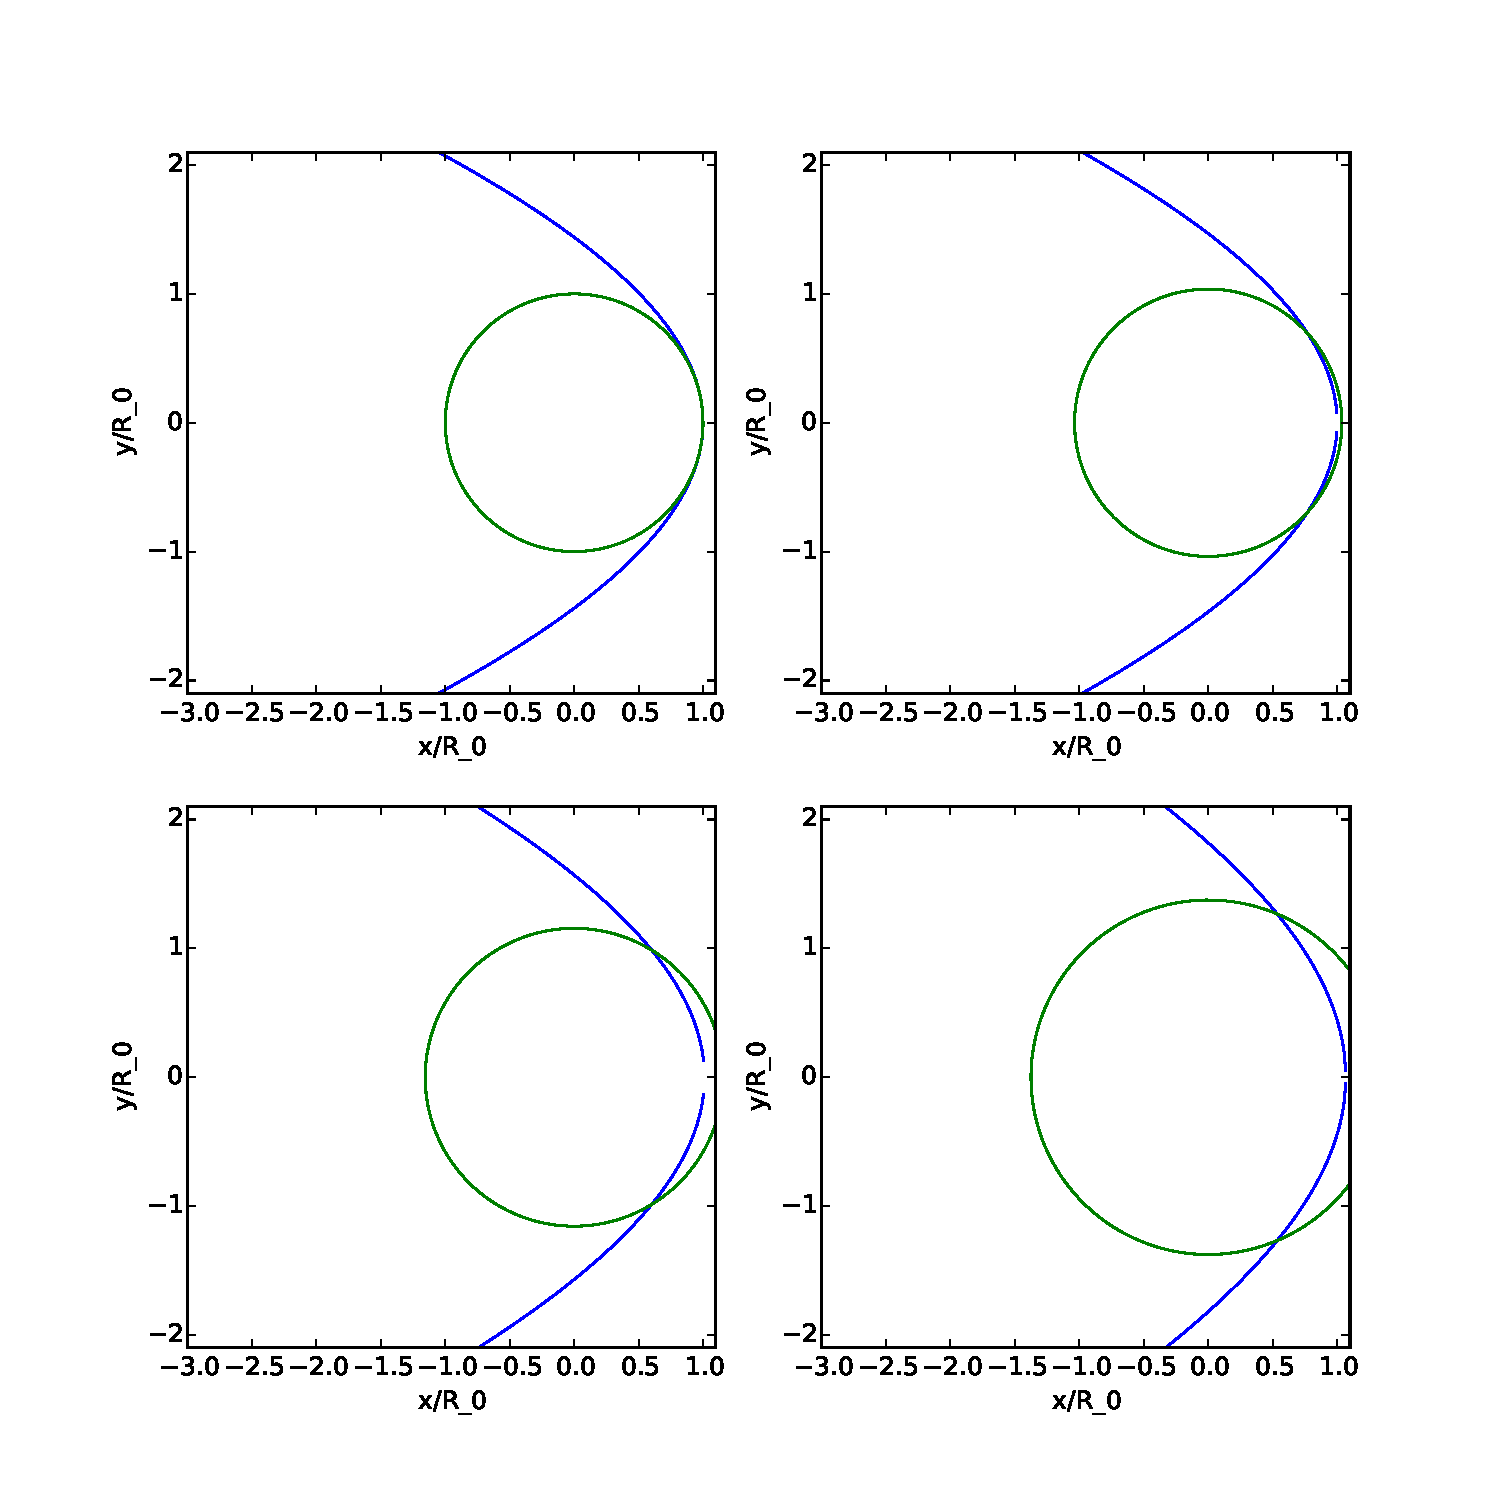
\includegraphics[width=0.8\linewidth]{conic2}
% \label{fig:conic2}
% \caption{Graphic example of the increasing of the projected radius of curvature with inclination}
% \end{figure*}

Using a space of parameters like figure \ref{fig:Apqp} we can compare models with observations of real bowshocks.

%The space parameter $A'$ vs $q'$ can be seen in figure (\ref{fig:Apqp}).%In this figure is assumed that we know the intrinsic Radius of curvature and $R_0$, which is not the case with
%real observations.

 
%%% Local Variables:
%%% mode: latex
%%% TeX-master: "proplyd-bowshocks"
%%% End:

